\documentclass[12pt]{report}
\usepackage[spanish]{babel}
\usepackage[utf8]{inputenc}
\usepackage{graphicx}
\usepackage{verbatim}
\usepackage{listings}
\usepackage{float}
\renewcommand*\thesection{\arabic{section}}

\begin{document}
	
	\begin{center}
		\textbf{Análisis de Algoritmos, Sem: 2018-1, 3CV1, Práctica 6, 10-2017}
		\newline
	\end{center}
	
	\begin{center}
		\begin{picture}(0,0) \put(-125,-55){
			\includegraphics[width=2.7cm]{../../IPNlogo.jpg}} 
		\end{picture}
		\LARGE Escuela Superior de Cómputo.\\
		Instituto Politécnico Nacional, México.\\
		\begin{picture}(0,0) \put(160,10){
			\includegraphics[width=2.7cm]{../../logoescom.png}} 
		\end{picture}
	\end{center}
	
	\begin{center}
		\Large Práctica 6: Problema del máximo subarreglo.\\
	\end{center}
	
	\begin{center}
		\textbf{Blancas Pérez Bryan Israel}\\
		orionmunecaycanica@gmail.com\\
	\end{center}
	
	
	\textbf{\large Resumen: }Implementar un algoritmo para encontrar el máximo subarreglo de una cadena de enteros, utilizando el paradigma "Divide y Vencerás", y compararlo con el algoritmo de fuerza bruta. \newline\\
	\textbf{\large Palabras Clave: } Divide y Vencerás, Máximo Subarreglo, Máximo Subarreglo Cruzado, Complejidad Computacional.\\
	

	\section{Introducción}
	En esta práctica se implementará un algoritmo orientado al paradigma Divide y Vencerás, para encontrar el máximo subarreglo. Aunque, como se verá en el desarrollo de esta práctica, existen otros métodos para resolver este problema en específico, y depende de nosotros encontrar el óptimo.\newpage
	

	\section{Conceptos Básicos}
	\textbf{Problema del máximo subarreglo.}\\
		
	El problema del subvector (o subarreglo), de suma máxima consiste en encontrar un subvector de una determinada longitud $m$ cuya suma sea máxima dentro de un vector de longitud $n$, con $m \leq n$. La forma de aplicar este algoritmo, consiste en obtener los segmentos de suma máxima correspondientes a las mitades izquierda y derecha del vector y a la parte central para, una vez calculados, elegir el máximo de los tres [1].\\	
	
		\textbf{\\}
		\begin{figure}[H]
			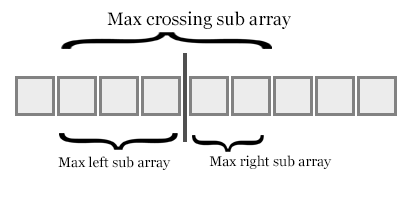
\includegraphics[width=12cm]{imagenes/1.png}
			\centering
			\caption{Maximum Subarray.}
			\centering
		\end{figure}
		
	\newpage
	
	\section{Experimentación y Resultados}	
	\textbf{Ejercicio 1.}\\
	Implementar el algoritmo de Máximo Subarreglo.\newline
	
	\textbf{i) Mediante gráficas, muestre que el algoritmo del Máximo Subarreglo Cruzado tiene orden de complejidad lineal.}\newline
	
	Pseudocódigo del algoritmo del Máximo Subarreglo Cruzado:
	\lstset{language=C, breaklines=true, basicstyle=\footnotesize}
	\lstset{numbers=left, numberstyle=\tiny, stepnumber=1, numbersep=10pt}
	\begin{lstlisting}
msc(A, bajo, medio, alto)
  int sumaizq = A[medio]
  suma = 0
    
  for i = medio to i = bajo
    suma += A[i]; 		
    if suma > sumaizq 	
      sumaizq=suma; 	
      min_izq=i;		
  
  int sumader=a[medio+1]
  suma = 0 
  
  for i = medio+1 to i = alto
    suma1 += A[i];		
    if suma1 > sumader	
      sumader = suma;	
      max_der=i;		

  return (max_izq, max_der, sumaizq + sumder);
	\end{lstlisting}
	
	Este algoritmo busca cual es la suma máxima que se puede lograr con los elementos del arreglo, considerando siempre que el subarreglo pase por en medio del arreglo original. En la figura 2, se observa el orden de complejidad del algoritmo, obtenido de manera experimental. La gráfica de color rojo, es la función $t(n)=5n$, demostrando así que el algoritmo del Máximo Subarreglo Cruzado, tiene orden $\theta (n)$.\newpage

	\begin{figure}[H]
		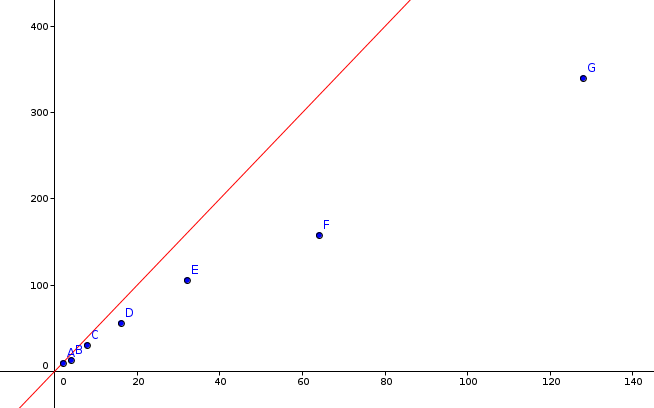
\includegraphics[width=12cm]{imagenes/2.png}
		\centering
		\caption{Máximo Subarreglo Cruzado.}
		\centering
	\end{figure}

	\textbf{ii)Demuestre analíticamente que el algoritmo del máximo subarreglo cruzado tiene complejidad lineal.}\newline
	
	\begin{table}[htbp]
		\begin{center}
			\begin{tabular}{|l|l|}
				\hline
				\multicolumn{2}{|c|}{Análisis del Algoritmo} \\ 
				\hline
				\textbf{} & \textbf{No. ejecuciones}\\
				\hline
				$1er \ for$ & $medio - bajo + 2$ \\ \hline
				$2do \ for$ & $alto -(medio + 1)+2$ \\ \hline			
			\end{tabular}
			\caption{Análisis del algoritmo.}
			\label{tabla:analisis1}
		\end{center}
	\end{table}
	Sumando el número de ejecuciones del 1er y 2do for, y considerando el tamaño total del arreglo igual a $n$, tenemos: \\
	$1er for + 2do for = alto - bajo +3= (alto - bajo + 1)+2= n + 2$\\
	
	$Por \ lo \ tanto \ Maximo \ Subarreglo \ Cruzado \  \epsilon \ \theta (n).$\\
	\newpage
	
	\textbf{iii) Mediante gráficas, muestre que el algoritmo del Máximo Subarreglo tiene orden de complejidad $\theta (n log(n))$.}\newline
	
Pseudocódigo del algoritmo del Máximo Subarreglo:
\lstset{language=C, breaklines=true, basicstyle=\footnotesize}
\lstset{numbers=left, numberstyle=\tiny, stepnumber=1, numbersep=10pt}
\begin{lstlisting}
ms(int *a, int bajo, int alto){
  if bajo = alto		
    return (bajo, alto, a[alto]) 
  else							
    medio = (bajo + alto) / 2;		
    (min_izq, max_der, suma_izq) = ms(a, bajo, medio);			
    (min_izq, max_der, suma_der) = ms(a, medio+1, alto);		
    (min_izq, max_der, suma_cruz) = msc(a, bajo, medio, alto);	
  
    if(suma_izq >= suma_der and suma_izq >= suma_cruz){
      return (min_izq, max_der, suma_izq)
    else if(suma_der >= suma_izq and suma_der >= suma_cruz){
      return (min_izq, max_der, suma_der)
    else 
      return (min_izq, max_der, suma_cruz)

\end{lstlisting}
	
	Como se puede ver en el pseudocódigo, este algoritmo implementa el paradigma Divide y Vencerás, puesto que va dividiendo el arreglo analizado una y otra vez, cada que se llama a si misma, hasta que solamente quede un arreglo de tamaño 1. Cuando se tengan las tres sumas de los subarreglos (suma\_izq, suma\_der y suma\_cruz), se comparan para determinar cuál es el mayor de ellos y retornar el indicado.\newline
	En la figura 3, se muestra la gráfica de los valores obtenidos de la ejecución del algoritmo implementado en el lenguaje C. La gráfica de color rojo, corresponde a la función $t(n) = 4 nlog(n)$, demostrando así, que el algoritmo esta acotado por dicha función, y por lo tanto tiene un orden de complejidad $\theta (n log n)$
	
	\begin{figure}[H]
		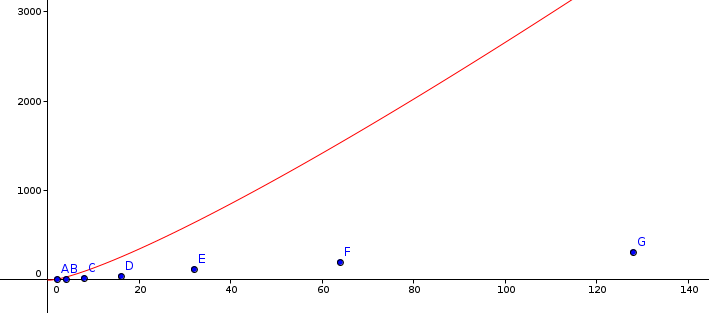
\includegraphics[width=12cm]{imagenes/3.png}
		\centering
		\caption{Máximo Subarreglo.}
		\centering
	\end{figure}
	
	\textbf{iv) Demuestre analíticamente que el algoritmo del Máximo Subarreglo tiene orden de complejidad $\theta (n log(n))$.}\newline
	\begin{table}[htbp]
		\begin{center}
			\begin{tabular}{|l|l|}
				\hline
				\multicolumn{2}{|c|}{Análisis del Algoritmo} \\ 
				\hline
				\textbf{Línea de Código} & \textbf{Orden de complejidad}\\
				\hline
				2-5 & $\theta (1)$ \\ \hline
				6 & $\theta (n/2)$ \\ \hline
				7 & $\theta (n/2)$ \\ \hline
				8 & $\theta (n)$ comprobado antes \\ \hline
				10-15 & $\theta (1)$ \\ \hline
			\end{tabular}
			\caption{Análisis del algoritmo.}
			\label{tabla:analisis3}
		\end{center}
	\end{table}\\
	Por lo tanto, se tiene una ecuación recursiva de la siguiente forma:
	
	$T(n) = \left \{ \begin{array}{c} C \ si \ n=1 \\ 2T(n/2)+\theta (n) \ si \ n \ > \ 1 \end{array}\right.$\\
	Aplicando el Teorema Maestro, se tiene $a=2, \ b=2 \ y \ f(n)=\theta (n)$. Luego $n^{log_{b}a}=n^{log_{2}2}=n$.\\
	Entonces $f(n)=\theta (n)$.\\
	Por lo tanto por el caso 2, del Teorema Maestro se tiene $T(n) \epsilon \ \theta (nlog_{2}(n))$
	\newpage
	
	\textbf{v) Implementar un algoritmo que resuelva el problema del máximo
		subarreglo utilizando fuerza bruta. Calcule su orden de complejidad analítica y experimentalmente.}\newline
	
Pseudocódigo del algoritmo del Máximo Subarreglo (Fuerza Bruta):
\lstset{language=C, breaklines=true, basicstyle=\footnotesize}
\lstset{numbers=left, numberstyle=\tiny, stepnumber=1, numbersep=10pt}
\begin{lstlisting}
ms(A,n)
  max=0			
  for i = 0 to i < n	
    suma=0	
    for  j = i to j < n
      suma += a[j]		
      if suma > max		
        max=suma;	

return max;
\end{lstlisting}

Este algoritmo es el más sencillo de implementar y de comprender, ya que se calcula todas las sumas posibles de todos los subarreglos que se pueden formar del arreglo original. El la figura 4, se muestra la gráfica de $T(n) \ vs \ n$, la gráfica de color rojo, corresponde a la función $T(n)=2n^{2}$, demostrando que este algoritmo tiene un orden de complejidad $\theta (n^{2})$.
	
	\begin{figure}[H]
		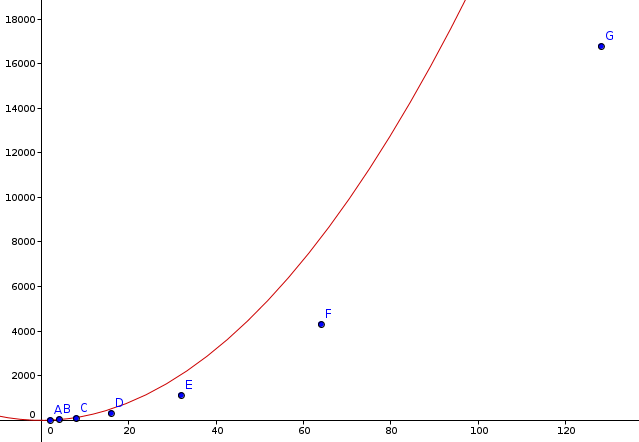
\includegraphics[width=12cm]{imagenes/4.png}
		\centering
		\caption{Máximo Subarreglo (Fuerza Bruta).}
		\centering
	\end{figure}	
	
Demostración analítica.\newline
	\begin{table}[htbp]
		\begin{center}
			\begin{tabular}{|l|l|}
				\hline
				\multicolumn{2}{|c|}{Análisis del Algoritmo} \\ 
				\hline
				\textbf{Línea de Código} & \textbf{Orden de complejidad}\\
				\hline
				3 & $\theta (n)$ \\ \hline
				5 & $\theta (n)$ \\ \hline
				2,4,6,7,8,10 & $\theta (1)$ \\ \hline
			\end{tabular}
			\caption{Análisis del algoritmo de fuerza bruta.}
			\label{tabla:analisis4}
		\end{center}
	\end{table}\\
	
	Como las lineas de código dentro del segundo for, tiene orden de complejidad constante, ese bloque tiene complejidad lineal.\newline
	Como existen dos for anidados, se aplica el teorema de la multiplicación, quedando: \newline
	$T(n)=\theta (n*n)$, correspondientes al orden de complejidad del primer y segundo for. Así entonces:
	$T(n)= \theta (n^{2})$\\

		$Por \ lo \ tanto \ , \ T(n) \epsilon \ \theta (n^{2})$\newpage

	
\section{Conclusiones}
Está práctica se me hizo muy sencilla, puesto que los algoritmos eran fáciles de implementar en un lenguaje de programación, y además, la lógica detrás de ellos no era tan compleja.\newline
Lo que me parece más relevante de esta práctica, es identificar el algoritmo óptimo para la solución de un problema, porque como bien sabemos, existen muchos algoritmos para resolver una solo problemática.\newpage 


\section{Anexo}

Resolver los siguientes problemas.\\

i) ¿Qué retorna la función de máximo subarreglo cuando todos los valores del arreglo son enteros negativos?.\\

\textbf{R: Retorna siempre sólo dos elementos, el elemento en la posición $n/2$, y $(n/2)+1$. Esto es porque como el se desea obtener el máximo subarreglo, cualquier número que le sumemos a los iniciales, hará más pequeño el valor de la suma total del subarreglo, contradiciendo el objetivo del algoritmo}.\\

\section{Bibliografía}

[1] https://es.wikipedia.org/wiki/Subvector\_de\_suma\_máxima\\
	
\end{document}